% !TeX root = ../my-thesis.tex
\chapter{Energieeffizientes Multithreading}
\section{Theoretische Einführung in die Parallelität}
Das Ziel hinter der Parallelisierung von Aufgaben ist die Beschleunigung der Laufzeit bei der Abarbeitung von Programmabläufen und die Minimierung der Wartezeiten des Prozessors. Solche Wartezeiten können entstehen, wenn während der Programmausführung Benutzereingaben nötig sind bevor die Ausführung fortgesetzt werden kann oder wenn neue Daten aus dem vergleichsweise langsamen Hauptspeicher nachgeladen werden müssen, da der prozessoreigene Cache nicht groß genug ist \cite[1135]{wolf2020}. Ohne Parallelität würden moderne Softwareanwendungen jeglicher Art nahezu unnutzbar werden. Einfache Vorgänge wie das Laden von Benutzerdaten aus einer lokalen Datenbank oder das downloaden von Bildern aus dem Netz, würden zum Einfrieren der Benutzeroberfläche führen, da bei sequentiellen Programmabläufen alle Aufgaben strikt hintereinander ausgeführt werden müssen. Android selbst wäre ohne Parallelität nicht umsetzbar, da Android's Architektur Multithreading und damit Parallelität voraussetzt.\todo{Erklärung}

Für die Realisierung von Parallelität haben sich mit der Evolution der Prozessortechnologie verschieden Ansätze und Techniken entwickelt. Jede dieser Techniken ist bis heute relevant und glänzt in unterschiedlichen Anwendungsfällen.

\underline{Pipelining}

Beim Pipelining wird die Ausführung von Befehlen in verschiedene Phasen aufgeteilt, welche jeweils durch eine eigene Ausführungseinheit bearbeitet werden. Sobald ein Befehl die aktuelle Phase abgeschlossen hat und zur nächsten Phase springt, kann bereits mit der Bearbeitung des nächsten Befehls, in der frei gewordenen Phase begonnen haben. In \autoref{fig:Pipeline} ist ein Beispiel einer 5-Phasen Pipeline veranschaulicht. Die Bearbeitung jeder Phase dauert im Optimalfall einen Taktzyklus, da andernfalls die Pipeline durch dies Phase geblockt werden kann, wie es in diesem Beispiel bei Befehl 3 während der Execute Phase der Fall ist. Ein großer Nachteil von Pipelining tritt bei häufigen Programmsprüngen auf, da bei jedem Sprung die komplette Pipeline geleert werden muss und alle Phasen, die bis dorthin vollendet wurden, verworfen werden und umsonst bearbeitet wurden. Dieser ist besonders bei größeren Pipelines kritisch \cite{pipelineElektro}.
\begin{figure}[H]
	\begin{center}	 
	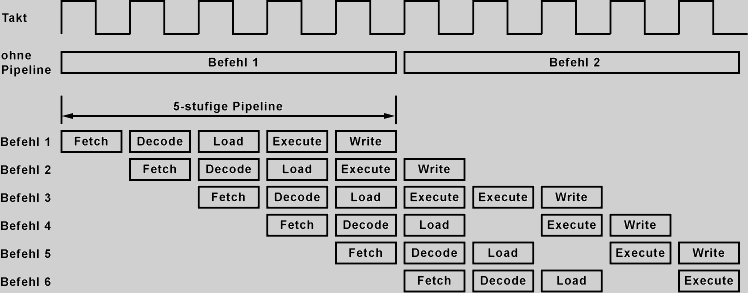
\includegraphics[scale=1]{Pipeline}
	\caption{Beispiel für eine 5-Phasen-Pipeline (Quelle: \cite{pipelineElektro})}
	\label{fig:Pipeline} 
	\end{center}
\end{figure}

\underline{simultanes Multi-Threading}

Ein Thread ist ein sequenzieller Ausführungspfaden innerhalb eines Prozesses, der ausgeführt wird. Bei Rechnern mit einem Prozessor kann zu einem Zeitpunkt immer nur ein Thread eines Prozesses gleichzeitig ausgeführt werde. Falls dieses Ausführung durch Ereignisse wie Speicherzugriffe oder Nutzereingaben warten muss, blockiert dieser Thread die \ac{cpu}. Durch sogenanntes simultanes Multi-Threading wird die verfügbare \ac{cpu} Zeit auf mehrere Prozesse und Threads aufgeteilt. Die \ac{cpu} kann dadurch zwischen den Threads hin und her springen und so längere Wartezeiten verhindern. Dies steigert die Effizienz der \ac{cpu} hinsichtlich der Laufzeit sowie des Energieverbrauchs \cite[877]{cplusplus}.

\underline{Hyper-Threading}

Die Technologie Hyperthreading wurde von Intel mit den Prozessoren Pentium 3, Pentium 4 und Xeon eingeführt. Hierbei wird wird der Durchsatz von Multithreaded-Anwendungen im Multitasking erhöht, indem sie die Auslastung der On-Chip-Ressourcen erhöht, die in der Intel-NetBurst-Mikroarchitektur verfügbar sind. Ein typischer Thread belastet nur etwa 35 \% der NetBurst-Ausführungsressourcen. Hyperthreading erhöht die Auslastung durch notwendige Logik und Ressourcen, die der CPU hinzugefügt werden. Für die Aufteilung der einkommenden Daten auf den freien Raum sorgen somit zwei logische Prozessoren, die vom Betriebssystem mittels klassischer Multiprocessing-Verfahren verwaltet werden \cite[1138]{wolf2020}. Somit stehen dem Rechner also 2 logische Rechenkern zur Verfügung trotz physischer Single Core \ac{cpu}. Dies bietet die Möglichkeit Speicherwartezeiten zu überbrücken. Wenn der erste Thread im Wartezustand ist, kann der Prozessor mithilfe des zweiten logischen Kerns in der Programmausführung fortfahren.

\underline{Multi-Core-Prozessor}

Bei Multi-Core Systemen handelt es sich um Prozessoren mit mehreren physischen Rechenkernen. Diese können voneinander unabhängig arbeiten und ermöglichen echte Parallelität. Alle Rechenkerne nutzen auch die schon genannten Techniken um möglichst effiziente Ergebnisse zu erhalten. Der Vorteil liegt hierbei nicht nur in der Steigerung der Geschwindigkeit. Mehrkernprozessoren können wesentlich geringer getaktet werden als Single Core Prozessoren und ermöglichen trotzdem erhöhte Laufzeitgeschwindigkeit bei geringerer Leistungsaufnahme und Wärmeentwicklung \cite{MulicoreElektro}. Es könnte die Annahme getroffen werden, dass mit steigender Rechenkernzahl auch die Leistung addiert wird. Sodass die neue Laufzeit im Multi-Core-Betrieb gleich der ursprünglichen Laufzeit mit einem Kern geteilt durch die Anzahl der Rechenkerne beträgt. In der Realität ist dies jedoch nicht umsetzbar, da verschiedene Faktoren diese Annahme begrenzen. Zunächst einmal wächst mit steigender Anzahl an Rechenkernen auch der Aufwand der Verwaltung durch das Betriebssystem. Außerdem ist es nicht einfach den Zugriff auf geteilte Speicherressourcen durch mehrere Rechenkerne zu synchronisieren. Die Laufzeit für parallele Prozesse setzt sich grob aus folgenden Anteilen zusammen.
\begin{aligneddescription}
\item[Rechenzeit] Zeit für die Durchführung von Berechnungen unter Verwendung von Daten im lokalen Speicher der einzelnen Prozessoren.
\item[Kommunikationszeit] Zeit für den Austausch von Daten zwischen Prozessoren.
\item[Wartezeit] Z.B. aufgrund ungleicher Verteilung von Last zwischen den Rechenkernen, Datenabhängigkeiten im Algorithmus oder Ein- und Ausgabe.
\item[Synchronisationszeit] Zeit für die Synchronisation beteiligter Prozesse und von Ressourcenzugriffen.
\item[Platzierungszeit] Zeit für die Allokation der Tasks auf die einzelnen Prozessoren, sowie eine mögliche dynamische Lastverteilung zur Programmlaufzeit.
\item[Startzeit] Zeit zum Starten der parallelen Threads auf allen Rechenkernen.
\end{aligneddescription}\cite[313]{parallelBook}

Viele Anwendungen können nur für kleine Bestandteile ihrer Ausführung von den Vorteilen eines Multi-core Systems profitieren, da die meisten Anwendungsfälle durch Nutzeraktionen bestimmt sind. Bei Programmabläufen mit strikt aufeinanderfolgenden Abhängigkeiten ist Parallelität ohnehin nicht möglich und resultiert in traditionell sequentielle Abläufe. Das Admahl'sche Gesetz beschreibt genau diese Grenze. So ist der Beschleunigungsfaktor, auch Speedup genannt, mit zusätzlichen Rechenkernen durch sequentielle Anteile eines Problems begrenzt \cite[314]{parallelBook}. Der Speedup $S_{ p }(n)$ wird durch \autoref{eq:Speedup} bestimmt. Dabei kennzeichnet $n$ die Problemgröße der Berechnung, $T_{ seq }(n)$ die Laufzeit der sequentiellen Ausführung und $T_{ p }(n)$ die Laufzeit der parallelen Ausführung mit $p$ Rechenkernen.

\begin{equation}\label{eq:Speedup}
S_{ p }(n) =\frac{ T_{ seq }(n) }{ T_{ p }(n) }
\end{equation}
\cite[314]{parallelBook}

Die Effizienz (\autoref{eq:Effizienz}) eines parallelen Programms gibt die relative Verbesserung des Speedups $S_{ p }(n)$ bezüglich der Anzahl $p$ der Prozessorkerne an. Diese Größen werden im Laufe dieses Kapitels für den Vergleich von Laufzeiteffizienz und Energieeffizienz in Abhängigkeit der Thread Anzahl verwendet.

\begin{equation}\label{eq:Effizienz}
E_{ p }(n) =\frac{ S_{ p }(n) }{p}
\end{equation}
\cite[316]{parallelBook}

Um Parallelität durch Multi-Core Systeme effektiv zu realisieren, müssen die 
\begin{itemize}
\item Beschleunigungsfaktor ($n_{ s }$)
\item Gesamtlaufzeit (Z)
\item Laufzeit für parallelisierbare Anteile ($Z_{ p }$)
\item Laufzeit für sequentielle Anteile ($Z_{ s }$)
\item Anzahl der Prozessoren ($n_{ p }$)
\item Zeitaufwand zur Verwaltung von Threads in Abhängigkeit
 von der Anzahl an Rechenkernen ($Z_{ 0(n_{ p }) }$)
\end{itemize}
\begin{equation}\label{eq:Amdahlsche Gesetz}
n_{ s }=\frac{ Z }{ Z_{ s } +Z_{ 0(n_{ p }) }+ \frac{ Z_{ p } }{ n_{ p } }} \leq \frac{ Z }{Z_{ s }  } = \frac{ Z }{ Z-Z_{ p } }
\end{equation}
In \autoref{eq:Amdahlsche Gesetz} ist das Amdahl‘sche Gesetz zu sehen

\section{Ein Base64 Encoder}
\section{Thread Pool Implementierung in Android}
\section{Messdatenerfassung}
\section{Auswertung und Erkenntnisse}